\section{An Operating System as One Process}\label{sec:model}

\Cref{sec:background} gave us a calculus of processes, equivalences that say what
an observer at each level sees, and one composition theorem per constructor. We now
use the calculus to write an operating system with interrupt handling as a single
process, following the example of \cref{fig:leak}: the secret is whether a disk
interrupt occurred. We first introduce the processes the system runs
(\cref{sec:pool}) and how they run together (\cref{sec:running}). That explains what
the system receives (\cref{sec:interface}) and what it emits
(\cref{sec:outputs}). We then give the rule that decides which process runs
(\cref{sec:state}). What is left open is the \emph{interrupt policy}
(\cref{sec:parameters}); \cref{sec:designs} gives two.

\subsection{The processes}\label{sec:pool}

The system runs six processes: three interrupt handlers, a scheduler, and two user
processes.

\paragraph{Handlers} The timer, disk and NOP handlers are copies of one process. A
handler run takes exactly \code{runtime} steps, and on its last step the handler
emits \code{Notify} to announce completion.

\paragraph{User processes} The public user process issues requests (\code{Get})
whose results the attacker sees. The private user process takes the disk handler's
output as input, and emits \code{Sys} when it has been notified of a disk event and
\code{Idle} otherwise.

\paragraph{Scheduler} When the scheduler runs, it proposes which user process runs
next.

\subsection{How the processes run together}\label{sec:running}

The six processes run side by side in a \emph{pool} (\cref{fig:system}), and only
one of them takes a step at a time. Each sits behind a switch, controlled by the
current process identifier (pid): a pid names one slot, whose process takes one
step, while every other slot emits \code{None} without moving. The pid is held in a
global state, which a state cell and a feedback loop thread around the pool.

\begin{figure}[t]
\centering
\begin{tikzpicture}[>=stealth, font=\scriptsize,
  slot/.style={draw, minimum width=2.3cm, minimum height=0.42cm, inner sep=0pt},
  outv/.style={minimum width=1.0cm, minimum height=0.42cm, inner sep=0pt,
    font=\ttfamily\scriptsize}]
% six slots and their outputs, on a common grid
\foreach \n/\l/\o [count=\k from 0] in
  {t/timer handler/None, d/disk handler/None, z/NOP handler/None,
   s/scheduler/None, v/private user/None, u/public user/Some o}
  {\node[slot] (\n) at (3.0, 1.05-0.42*\k) {\l};
   \node[outv] (o\n) at (5.15, 1.05-0.42*\k) {\o};
   \draw[->] (\n.east) -- (o\n.west);}
\node[draw, dashed, rounded corners=2pt, fit=(t)(u), inner sep=3pt] (pool) {};
\node[draw, rounded corners=2pt, fit=(ot)(ou), inner sep=2pt] (tuple) {};
\node[anchor=south] at (pool.north) {pool: six slots in \texttt{par}};
\node[anchor=south] at (tuple.north |- pool.north) {six-tuple};
% global state, vertically centred on the pool
\node[draw, rounded corners=2pt, minimum width=1.3cm, minimum height=1.1cm,
  align=center] (sta) at (0.35, 0 |- pool.center) {global\\state};
\draw[->] (-1.25, 0 |- sta.center) -- node[above] {interrupt} (sta.west);
\draw[->] (sta.east) -- node[above] {pid} (pool.west |- sta.east);
\draw[->] (tuple.east) -- ++(0.5,0) node[right] {out};
\draw[->] ($(tuple.east)+(0.25,0)$) |- ($(pool.south)+(0,-0.35)$) -|
  node[pos=0.25, below] {fed back (\texttt{loop})} (sta.south);
\end{tikzpicture}
\caption{The model. An interrupt only updates the global state. The state's pid
  selects one slot, which takes a step and emits \texttt{Some o}; every other slot
  emits \texttt{None}. Because the slots are composed with \texttt{par}, their
  outputs form a six-tuple, which is emitted and fed back to update the state.}
\label{fig:system}
\end{figure}

\subsection{Inputs}\label{sec:interface}

The system receives interrupts. Its input type \code{T_in} has two values, the timer
interrupt and the disk interrupt. An interrupt goes to the global state, where it
marks itself pending in the interrupt controller. The controller has one more
entry, for the NOP handler, which no external interrupt raises; the sliced policy of
\cref{sec:sliced} sets it pending itself, to use the NOP handler as filler.

The disk interrupt is the secret. The input equivalence \m{in_equiv} makes it, and
only it, unobservable to the attacker; otherwise interrupts are related only when
equal:
\begin{align*}
\mathit{ir} \doteq_\ell \unobs &\iff \mathit{ir} = \mathsf{Disk} \wedge \ell = \Lo, \\
\mathit{ir} \doteq_\ell \mathit{ir}' &\iff \mathit{ir} = \mathit{ir}' \vee
  (\mathit{ir} \doteq_\ell \unobs \wedge \mathit{ir}' \doteq_\ell \unobs).
\end{align*}

\subsection{Outputs}\label{sec:outputs}

By the rule for \code{par} (\cref{fig:semantics}), the pool emits the
outputs of all its slots together. So the system emits a six-tuple of options, the output
type \code{T_out}, with exactly one \code{Some} on each step. The output therefore
records not only what was computed but also \emph{who ran}: the schedule is part of
what the system emits. \Cref{fig:slots} shows what we intend to hide from the
attacker in each position. The exact output equivalence, and why the proof forces
its shape, come in \cref{sec:equivs}.

\begin{figure}[t]
\centering
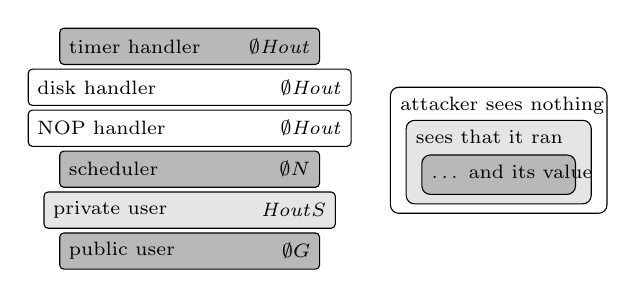
\begin{tikzpicture}[font=\scriptsize,
  proc/.style={draw, rounded corners=1.5pt, minimum width=4.1cm,
    minimum height=0.46cm, inner sep=1pt},
  % indented on both sides like the nested boxes of the key
  hid/.style={proc, fill=white},
  ran/.style={proc, fill=black!10, minimum width=3.7cm},
  val/.style={proc, fill=black!28, minimum width=3.3cm}]
% the processes, in the order of Fig.~3, shaded by what the attacker learns
\foreach \s/\k/\n/\t in
  {val/0/timer handler/{\Proc{\emptyset}{\mathit{Hout}}},
   hid/1/disk handler/{\Proc{\emptyset}{\mathit{Hout}}},
   hid/2/NOP handler/{\Proc{\emptyset}{\mathit{Hout}}},
   val/3/scheduler/{\Proc{\emptyset}{\mathbb{N}}},
   ran/4/private user/{\Proc{\mathit{Hout}}{S}},
   val/5/public user/{\Proc{\emptyset}{G}}}
  {\node[\s] (p\k) at (0, -0.52*\k) {};
   \node[anchor=west] at (p\k.west) {\n};
   \node[anchor=east] at (p\k.east) {$\t$};}
% key: the shades as nested sets
\begin{scope}[shift={(2.55,-0.52)}]
\draw[rounded corners=3pt, fill=white] (0,0) rectangle (2.75,-1.6);
\draw[rounded corners=3pt, fill=black!10] (0.2,-0.42) rectangle (2.55,-1.48);
\draw[rounded corners=3pt, fill=black!28] (0.4,-0.86) rectangle (2.35,-1.36);
\node[anchor=north west] at (0,0) {attacker sees nothing};
\node[anchor=north west] at (0.2,-0.42) {sees that it ran};
\node[anchor=north west] at (0.4,-0.86) {\dots\ and its value};
\end{scope}
\end{tikzpicture}
\caption{The six processes, with their types, shaded by what the attacker learns
  of each (key on the right). $\mathit{Hout} = \{\mathtt{Notify},
  \mathtt{Nothing}\}$ is the handler output, which the private user reads from the
  disk handler; $S = \{\mathtt{Sys}, \mathtt{Idle}\}$, $G = \{\mathtt{Get}\}$, and
  the scheduler emits a pid.}
\label{fig:slots}
\end{figure}
\subsection{When does a handler run?}\label{sec:state}

Besides the current pid, the global state holds an interrupt controller with a
\emph{pending} bit and a \emph{mask} bit for each handler: timer, disk and NOP. A
handler can be started when its entry is pending and not masked; if several can,
the timer goes first, then the disk, then NOP. Handlers cannot be interrupted: starting one sets all masks.

The state changes once per event. On an interrupt, \m{set_pending} sets that
interrupt's pending bit. On a pool output, \m{check_scheduler} adopts the pid the scheduler
proposed, if the scheduler ran; then \code{service_policy}, part of the interrupt
policy (\cref{sec:parameters}), reacts to the output; and finally \m{initiate_next} decides
who runs next by a priority rule:
\begin{enumerate}
\item if a handler is running, it continues;
\item otherwise, if a handler can be started, it starts;
\item otherwise, if a handler has just finished, control returns to the user
  process it interrupted, or to the scheduler if a reschedule was requested;
\item otherwise, the current process continues.
\end{enumerate}
Just before the choice, \m{initiate_next} applies \m{restore_invariant}, which
\cref{sec:parameters} explains.
Appendix~\ref{app:model} gives the code.

This is enough to see the leak of \cref{fig:leak}. With the disk unmasked, a disk
interrupt sets its pending bit. At the next output, rule 2 applies and the disk
handler starts at once, and for the \code{runtime} steps of the handler the public
user's slot emits \code{None}.

\subsection{The interrupt policy}\label{sec:parameters}

Together, these parts form the generic model
\begin{lstlisting}
model runtime init_policy service_policy
      restore_invariant p_pub p_priv p_sched
  : Proc T_in T_out
\end{lstlisting}
(\m{model}, written out in Appendix~\ref{app:model}). Its first argument,
\code{runtime}, is the handler length, and its last three are the scheduler and the
two user processes. The pool, the layout of the state, \m{set_pending},
\m{check_scheduler} and \m{initiate_next} are fixed. The remaining three arguments
are where models differ:
\begin{itemize}
\item \code{init_policy}, the initial state. Its masks decide which interrupts can be
  serviced before anything has happened.
\item \code{service_policy}, which runs on each pool output, before
  \m{initiate_next}. It is the only place that sees a handler announce
  completion, and so the only place masks can be reopened: it decides when the next
  handler becomes eligible.
\item \m{restore_invariant}, which \m{initiate_next} applies just before choosing.
  It writes into the state an invariant that the other two already maintain, for
  the benefit of the proof (\cref{sec:restore}).
\end{itemize}
The first two decide \emph{when a handler may run}, and together we call them the
\emph{interrupt policy}. The third is not part of it: it never changes a state the
model reaches (\cref{thm:noop}), and it is the identity where the proof needs no
help. \Cref{tab:designs} gives all three for both policies.
